\section{Situazione esistente}

\subsection{App Economy}
  
\begin{figure}[h!]
  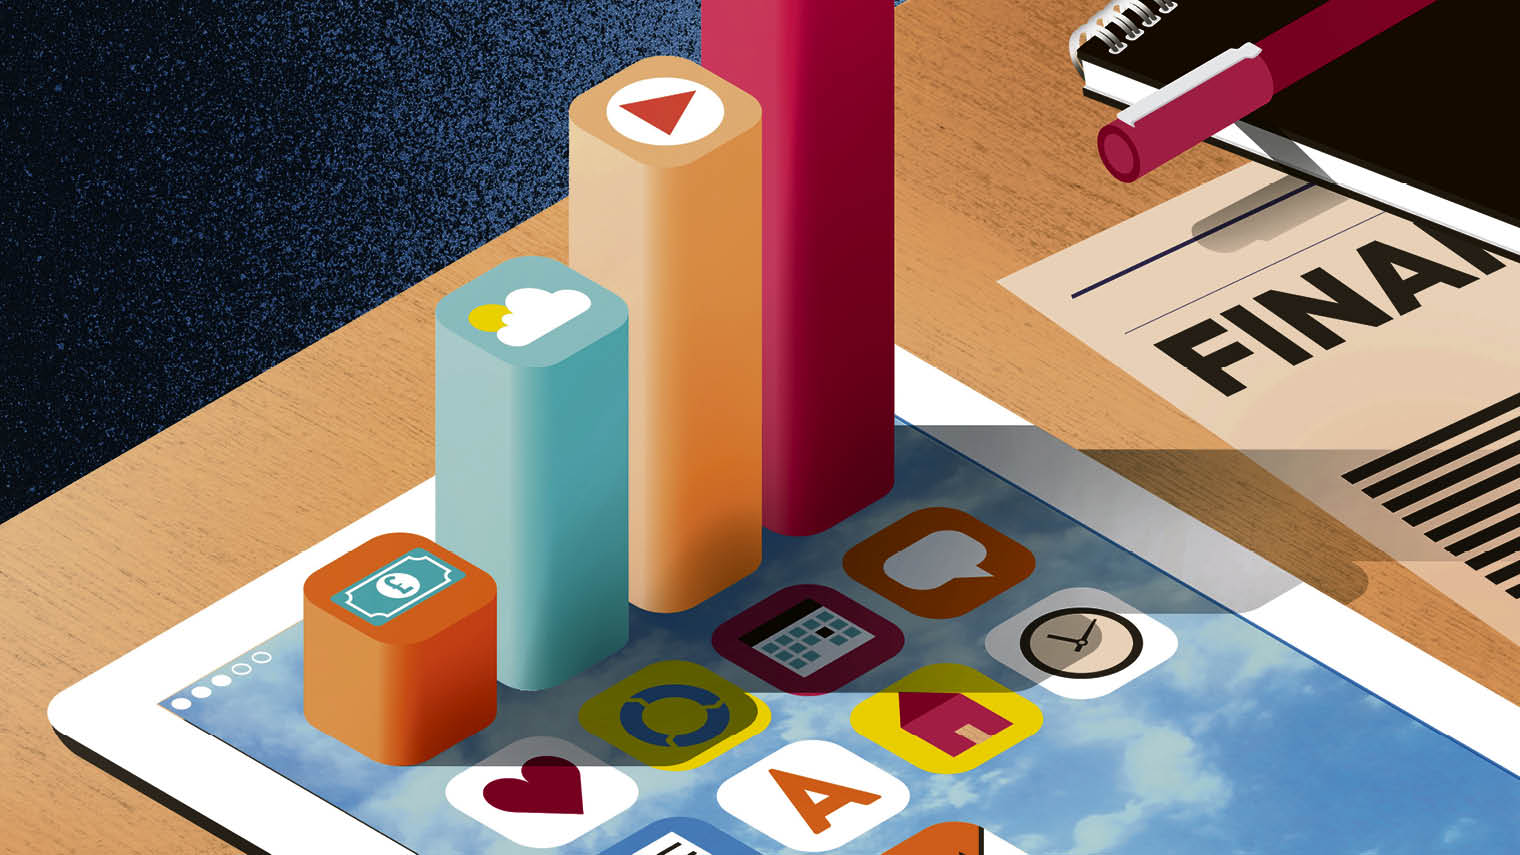
\includegraphics[width=\linewidth]{images/The-App-Economy.jpg}
  \caption{App Economy}
  \label{fig:appEconomy1}
\end{figure}
  
Non vi è forse modo di descrivere la società attuale e questo periodo storico senza valutare l'importanza dello sviluppo tecnologico che ci ha portato nell'\textit{Era dell'Informazione}.
La rivoluzione tecnologica che sta avvenendo in questi anni, specialmente a partire dagli Novanta, ha portato la connessione globale ad internet ad assumere un ruolo essenziale in ogni aspetto della società moderna e della nostra vita.

È cambiato drasticamente il modo con cui le persone accedono alle informazioni, che siano queste di tipo personale o di tipo economico.
Allo stesso modo si sono dovute adeguare le strategie di tutte quelle aziende che hanno visto cambiare in maniera drastica il proprio mercato, invaso molto volte da tecnologie sempre diversificate e innovative.

Secondo Paul Mason, è stata la dottrina economica degli ultimi decenni della nostra epoca che, da una parte ha avuto il merito di promuovere la più grande ondata di sviluppo economico che il mondo abbia mai visto, ma dall’altra ha portato a mercati incontrollatie a vorticosi cambiamenti sociali innescati dalla tecnologia.
Allo stesso modo si sono diffusi concetti come i progetti open-source, la sharing economy o le licenze creative commons che hanno portato ad uno stravolgimento di molti mercati dove tante aziende hanno dovuto rivedere la propria business strategy. \autocite{POSTCAPITALISMO}

Primi su tutti sono diventati di fondamentale importanza i concetti di e-commerce e marketing digitale, fortemente spinti dalle tecnologie e dalla nuova possibilità di accedere ad una risorsa comune (internet) da parte della maggior parte della persone anche di cultura, età e ambienti sociali diversi.
Diventa quindi fondamentale l'Application Economy: lo sviluppo e l'utilizzo di applicazioni mobile multipiattaforma per raggiungere gli utenti consumatori.
Questa strategia può essere applicata in ambito di marketing per pubblicizzare un proprio prodotto, fidelizzare il consumatore alla propria azienda e mantenere una propria immagine in un sistema in cui l'idea che i consumatori hanno dell'azienda è fondamentale.

Forse ancora in via di sviluppo ma ormai più diffuso è l'e-commerce, la possibilità di fare acquisti online, che ormai sta lentamente, ma inesorabilmente, spostandosi sui device mobile.
Proprio in questi ultimi anni tutti i principali protagonisti del mondo software hanno presentato la propria visione delle vendite online, affiancando anche i propri sistemi di pagamento online tramite device mobile.

\subsection{Ecosistema MyGelato}

L'ecosistema MyGelato si pone proprio all'interno di questo contesto, ad unire le strategie di marketing dell'azienda produttrice Carpgiani e delle singole gelaterie convenzionate; insieme alla possibilità di comprare, regalare e utilizzare dei coupon che permetto l'acquisto online di gelati.

È un progetto di piattaforma web e mobile che si rivolge al pubblico dei gelatieri e dei consumatori di gelato. Gli obiettivi commerciali sono diversi, primi tra i quali quello di incentivare la compravendita di gelati tramite il sistema di coupons digitali e quello di promuovere il consumo di gelato tramite offerte, fornendo anche ai gelatieri un sistema semplice ed efficace per pubblicizzare il proprio negozio.


\subsection{Stato dell’Arte dell’Applicazione Android}
\newpage